\section{Contexto}\label{sec:contexto}

Como se observa en la Figura\ref{fig:area_responsabilidad_armada}, el Uruguay, tiene asignada como región de responsabilidad, un segmento de la Zona 5 – Atlántico Sudoccidental, 
zona que comparte con la Rep. Argentina, la Rep. Federativa del Brasil y el Reino Unido. Esta área, que limita en su extremo Este \footnote{Longitud 010º W} con el área de responsabilidad de Sudáfrica, 
representa una superficie aproximada de 516.000 millas náuticas cuadradas\footnote{Esto equivale a \(1.770.000\ \text{km}^2\)}, equivalente a unas 10 veces el tamaño de la superficie terrestre de nuestro país.\\

\begin{figure}
    \centering
    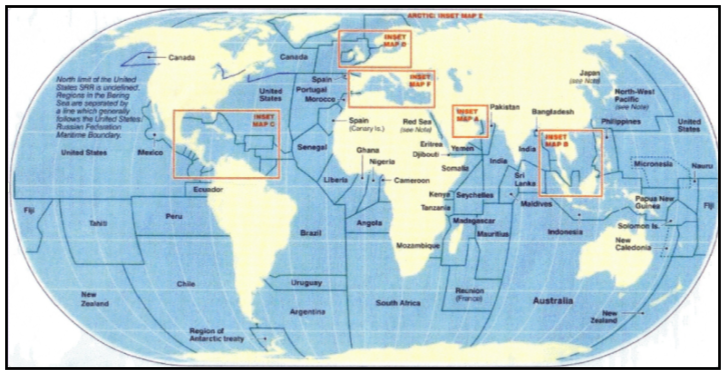
\includegraphics[width=\textwidth]{../imagenes/secciones/2-descripcion-del-problema-y-solucion/Regiones De Responsabilidad SAR.png} % Ancho total del texto
    \caption{Área de responsabilidad de la Armada Nacional}
    \label{fig:area_responsabilidad_armada}
\end{figure}


\FloatBarrier
